\documentclass{beamer}
\usepackage[utf8]{inputenc}
\usepackage[english]{babel} % Adds processing for some simple special characters.

% Packages for better page formatting and nice footnotes. %

\usepackage{fancyhdr} % Headers.
\usepackage{multicol} % Columns.

\renewcommand{\thefootnote}{\fnsymbol{footnote}}

% Utilities for fine-grained control over image insertion. %

\usepackage{graphicx} % Insert images.
\usepackage{float} % Images float in document environment.
\usepackage{wrapfig} % Image/tables in multicols with \wrapfigure or \wraptable.
\usepackage[justification=centering]{caption} % Captions for single images.
\usepackage{subcaption} % Captions for simultaneous images.
\graphicspath{{./img/}}

% Some utilities for scientific and mathematical writing. %

\usepackage{siunitx} % Formatting for numbers with SI units.
\usepackage{amsmath} % Astronomical symbols.
\usepackage{isotope} % Nice markup syntax for chemical symbols.
\usepackage{xfrac}   % Slant fractions and other utilities.
\usepackage{lipsum}  % Generate pseudo-text for formatting.
\usepackage{listings}

% Utilities for manual kerning adjustment. %

\newcommand\K{\kern.05em} % Small amount of kerning.
\newcommand\KK{\kern.1em} % Medium amount of kerning.
\newcommand\KKK{\kern.2em} % Large amount of kerning.
\newcommand\KKKK{\kern.3em} % Very large amount of kerning.

% Utilities for Beamer slides. %

% \usetheme{gemini}
\usecolortheme{mit}
\usepackage{epstopdf}
\setbeamertemplate{navigation symbols}{}

% Bibliography and referencing style.

\usepackage[backend=bibtex,style=phys,sorting=nyt]{biblatex} % Use style=draft for troubleshooting.
\addbibresource{references.bib}

% Title and author for title page. %

\title{Properties of AGN Host Galaxies}
\author{A. Wheaton}
\institute[UoE]{
\includegraphics[width=0.4\textwidth]{crest}\vspace{1em}}
\date{\today}

\begin{document}

\begin{frame}
  \titlepage
\end{frame}

\begin{frame}{Project Aims}
  \begin{table}
    \centering
    \resizebox{\textwidth}{!}{
    \begin{tabular}
      {| l | c | c | c | c | c | r |}
      \hline
      TDE         & Host Galaxy               & RA           & Dec          & Mag & z        \\
      \hline
      AT2019qiz   & WISEA J044637.88-101334.9 & 04:46:37.880 & -10:13:34.90 & 15  & 0.01513  \\
      AT2019azh   & KUG 0810+227              & 08:13:16.945 & +22:38:54.03 & 15  & 0.022    \\
      AT2018hyz   & WISEA J100650.83+014133.4 & 10:06:50.871 & +01:41:34.08 & 17  & 0.04573  \\
      AT2019dsg   & WISEA J205702.96+141216.2 & 20:57:02.974 & +14:12:15.86 & 15  & 0.0512   \\
      iPTF16fnl   & iPTF16fnl                 & 00:29:57.010 & +32:53:37.24 & 16  & 0.018    \\
      AT2019ahk   & WISEA J070011.40-660224.7 & 07:00:11.546 & -66:02:24.14 & 17  & 0.026211 \\
      ASASSN-15oi & ASASSN-15oi               & 20:39:09.18  & -30:45:20.10 & 16  & 0.0484   \\
      AT2018fyk   & LCRS B224721.6-450748     & 22:50:16.090 & -44:51:53.50 & 17  & 0.06     \\
      ASASSN-14li & ASASSN-14li               & 12:48:15.23  & +17:46:26.44 & 15  & 0.0206   \\
      ASASSN-14ae & ASASSN-14ae               & 11:08:40.12  & +34:05:52.23 & 17  & 0.0436   \\
      \hline
    \end{tabular}
    }
    \caption{The XSHOOTER targets on tidal disruption events.}
  \end{table}
  \begin{itemize}
    \item Investigate the statistical behaviour of the star formation in the host galaxies of tidal disruption events and active galactic nuclei (AGN).
  \end{itemize}
\end{frame}

\begin{frame}{Active Galactic Nuclei (AGN)}
  \section{Key Features}
  \begin{itemize}
    \item Compact, highly luminous nuclear region.\pause % From 10^35 W to 10^42 W, Milky Way core is 10^10 W.
    \item Broad spectral energy distribution.\pause % Non-stellar emission which is inexplicable by blackbody radiation.
    \item Strong (and sometimes broad) emission lines.\pause % Which if due only to the Doppler effect, imply gas motions of $v = 10000 km/s$.
    \item Variability over short timescales. % Minutes to days, in some cases a few years.
    % \item Upper bound on size $\approx 100 pc$ \cite{Peterson_1997} % Determined by spatial resolution, but requires 10% galactic mass to be central
    % \item For smaller $r$, need extraordinary energy production.\cite{Peterson_1997}
  \end{itemize}
\end{frame}

\begin{frame}{Active Galactic Nuclei (AGN)}
  \begin{figure}
    \centering
    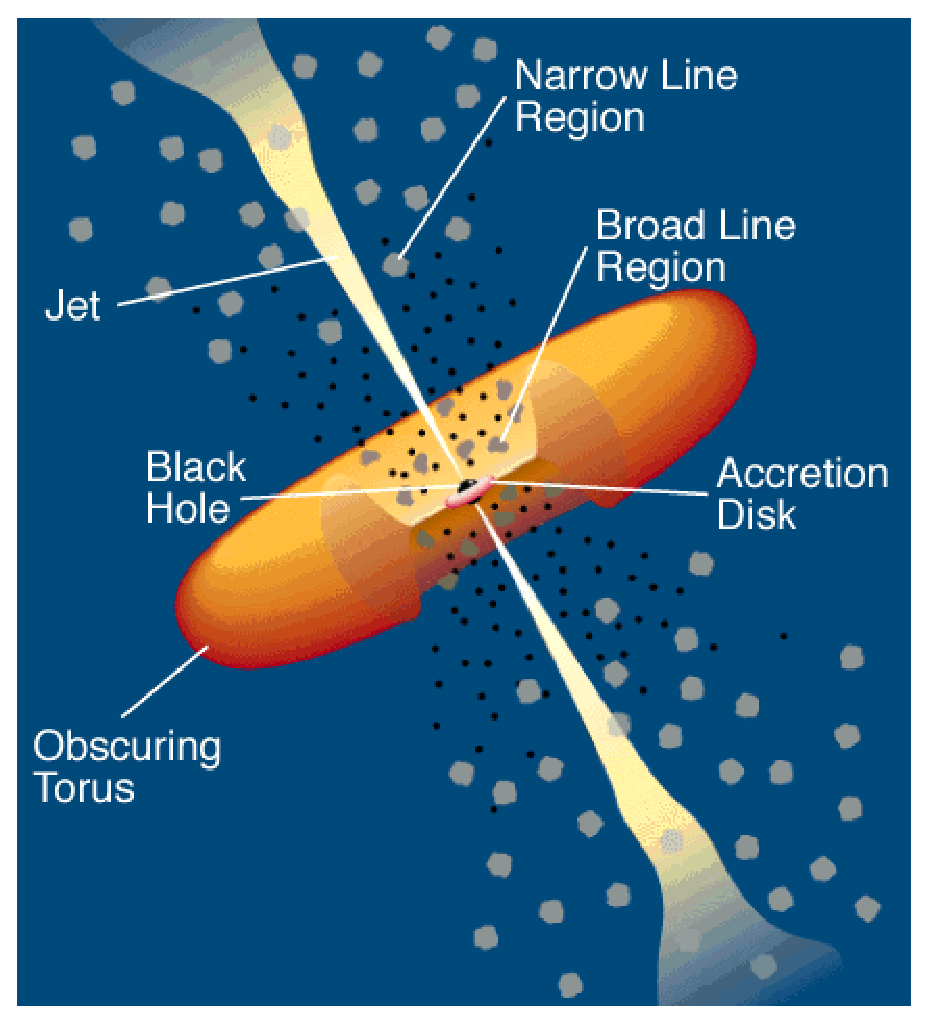
\includegraphics[width=0.5\textwidth]{agn_model}
    \caption{Accretion of matter onto surface of a black hole. Image adapted from Urry and Padovani 1995.\cite{Urry_1995}}
  \end{figure}
\end{frame}


\begin{frame}{The Starburst-AGN Connection}
  \begin{figure}
    \centering
    \includegraphics[width=0.5\textwidth]{image--002}
    \caption{Strong relationship between star formation and black hole mass. Image adapted from Veilleux 2008.\cite{Veilleux_2008}}
  \end{figure}
  \pause
  \begin{itemize}
    \item Cosmologically important impact on galaxy formation and evolution.
  \end{itemize}
\end{frame}

\begin{frame}{Possible mechanisms?}
  \begin{itemize}
    \item Gas or radiation pressure from starbursts and/or AGN-drive wind shuts off  black hole fuel supply.\pause
    \item Direction of causation unclear.\pause
    \item AGN is a possible source of quenching.\pause
    \item Need more information...
  \end{itemize}
\end{frame}

\begin{frame}{The BAGPIPEs Module}
  \begin{itemize}
    \item Bayesian Analysis of Galaxies for Physical Inference and Parameter EStimation.\pause
    \item Simulation of galactic spectra from SFH.\pause
    \item Fit real spectra to plausible SFH.
  \end{itemize}
\end{frame}

\begin{frame}{The BAGPIPEs Module}
  \begin{figure}
    \centering
    \includegraphics[width=0.9\textwidth]{model020_sfh}
    \includegraphics[width=\textwidth]{model020_spectrum}
    \caption{Simulated SFH and spectrum.}
  \end{figure}
\end{frame}

\begin{frame}{The BAGPIPEs Module}
  \begin{figure}
    \centering
    \includegraphics[width=0.9\textwidth]{host_hyz_specwerr_fit}
    \includegraphics[width=0.9\textwidth]{host_hyz_specwerr_sfh}
    \caption{Observed and fitted spectrum, with inferred SFH.}
  \end{figure}
\end{frame}

\begin{frame}{Stellar Population Dating}
  \begin{figure}
    \centering
    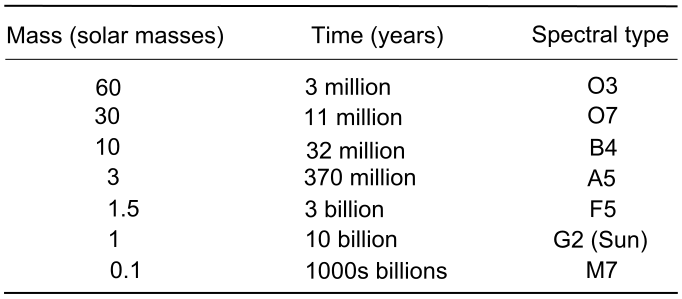
\includegraphics[width=0.9\textwidth]{lifetimes}
    \caption{Stellar lifetimes and spectral type.}
  \end{figure}
  \begin{itemize}
    \item Poor temporal resolution in SFR beyond 1 billion years.
  \end{itemize}
\end{frame}

\begin{frame}{Stellar Population Dating}
  \begin{figure}
    \centering
    \includegraphics[width=0.9\textwidth]{Screenshot.png}
    \caption{Number density of spectral types. Table adapted from Glenn 2001.\cite{Glenn_2001}}
  \end{figure}
  \begin{itemize}
    \item Poor temporal resolution beyond ~1 billion years.
  \end{itemize}
\end{frame}

\begin{frame}{Stellar Population Dating}
  \begin{itemize}
    \item Solution?\pause \KKKK Parameterise metallicity as well.\pause
    \item How do Lyman and Balmer series lines evolve with starburst age?
    \item What about other metal lines?
  \end{itemize}
\end{frame}

\begin{frame}{}
  \begin{figure}
    \centering
    \includegraphics[width=\textwidth]{figure}
    \caption{Variance in flux, over starburst evolved from z=2.2 to z=0.01.}
  \end{figure}
\end{frame}

\begin{frame}{}
  \begin{figure}
    \centering
    \includegraphics[width=\textwidth]{figure1}
    \caption{Deltas in flux, over starburst evolved from z=2.2 to z=0.01.}
  \end{figure}
\end{frame}

\begin{frame}{SFH Inference - What is possible?}
  \begin{itemize}
    \item Blind fitting of spectra with known priors.\pause
    \item Fitting multiple SFH forms.\pause
    \item Iterative fitting.
  \end{itemize}
\end{frame}

\begin{frame}{Future Plans}
  \begin{table}
    \centering
    \resizebox{\textwidth}{!}{
    \begin{tabular}
      {| l | c | c | c | c | c | r |}
      \hline
      TDE         & Host Galaxy               & RA           & Dec          & Mag & z        \\
      \hline
      AT2019qiz   & WISEA J044637.88-101334.9 & 04:46:37.880 & -10:13:34.90 & 15  & 0.01513  \\
      AT2019azh   & KUG 0810+227              & 08:13:16.945 & +22:38:54.03 & 15  & 0.022    \\
      AT2018hyz   & WISEA J100650.83+014133.4 & 10:06:50.871 & +01:41:34.08 & 17  & 0.04573  \\
      AT2019dsg   & WISEA J205702.96+141216.2 & 20:57:02.974 & +14:12:15.86 & 15  & 0.0512   \\
      iPTF16fnl   & iPTF16fnl                 & 00:29:57.010 & +32:53:37.24 & 16  & 0.018    \\
      AT2019ahk   & WISEA J070011.40-660224.7 & 07:00:11.546 & -66:02:24.14 & 17  & 0.026211 \\
      ASASSN-15oi & ASASSN-15oi               & 20:39:09.18  & -30:45:20.10 & 16  & 0.0484   \\
      AT2018fyk   & LCRS B224721.6-450748     & 22:50:16.090 & -44:51:53.50 & 17  & 0.06     \\
      ASASSN-14li & ASASSN-14li               & 12:48:15.23  & +17:46:26.44 & 15  & 0.0206   \\
      ASASSN-14ae & ASASSN-14ae               & 11:08:40.12  & +34:05:52.23 & 17  & 0.0436   \\
      \hline
    \end{tabular}
    }
    \caption{The XSHOOTER targets on tidal disruption events.}
  \end{table}
  \begin{itemize}
    \item Compare SFH of TDE galaxies with Hubble analogues, and Seyferts.
  \end{itemize}
\end{frame}

\begin{frame}{References}
  \printbibliography
\end{frame}

\end{document}
